\documentclass[first=orange,second=purple,logo=redexc]{aaltoslides}
%\documentclass{aaltoslides} % DEFAULT
%\documentclass[first=purple,second=lgreen,logo=redque,normaltitle,nofoot]{aaltoslides} % SOME OPTION EXAMPLES

\usepackage[latin9]{inputenc}
\usepackage[T1]{fontenc}
\usepackage{graphicx}
\usepackage{amssymb,amsmath}
\usepackage{url}
\usepackage{lastpage}
\usepackage{array}
\usepackage{amsbsy}
\usepackage{multirow}
\usepackage[absolute,overlay]{textpos}


\newcolumntype{x}[1]{%
>{\centering\hspace{0pt}}p{#1}}%

\title{Multiresolution Mixture Modeling using \\Merging of Mixture Components}

\author[Prem Raj Adhikari]{ \underline{Prem Raj Adhikari}$^{1,2}$, Jaakko Hollm\'en$^{1,2}$ }
\institute[ICS]{ \hspace{0.5mm} Parsimonious Modelling Research Group in \\
$^{1}$Department of Information and Computer Science\\
\hspace{1.5mm}Aalto University School of Science, Finland\\
$^{2}$Helsinki Institute for Information Technology (HIIT) \\
%\hspace{1.5mm}Helsinki, Finland  \\
\hspace{1.5mm}\{prem.adhikari,jaakko.hollmen\}@aalto.fi }
\aaltofootertext{Multiresolution Mixture Modeling using Merging of Mixture Components} {Asian Conference on Machine Learning (ACML 2012)}{November 4--6,  \insertframenumber/\inserttotalframenumber}
\date{November 2--4, 2012}
\makeatletter

\begin{document}
%%%%%%%%%%%%%%%%%%%%%%%%%%%%%%%%%%%%%%%%%%%%%%%%%%%%%%%%%%%%%%%%%%%%%%%%%%%%%%%%%%%%%%%%%%%%%

\aaltotitleframe

%%%%%%%%%%%%%%%%%%%%%%%%%%%%%%%%%%%%%%%%%%%%%%%%%%%%%%%%%%%%%%%%%%%%%%%%%%%%%%%%%%%%%%%%%%%%%

% \begin{frame}
%   \frametitle{Outline}
%   \tableofcontents%[pausesections]
% 
% \end{frame}

% %%%%%%%%%%%%%%%%%%%%%%%%%%%%%%%%%%%%%%%%%%%%%%%%%%%%%%%%%%%%%%%%%%%%%%%%%%%%%%%%%%%%%%%%%%%%%

\begin{frame}{Management Summary}
\begin{itemize} \setlength{\itemsep}{6.5mm}
  \item The multiresolution data 
  \item Mixture Models of multiresolution data
  \item Experiments on two chromosomal aberrations datasets
  \item Summary and Conclusions
\end{itemize}
\end{frame}

%%%%%%%%%%%%%%%%%%%%%%%%%%%%%%%%%%%%%%%%%%%%%%%%%%%%%%%%%%%%%%%%%%%%%%%%%%%%%%%%%%%%%%%%%%%%%%


% 
% \begin{frame}{Exponential Growth of Biological Data}
% 
% \vspace{-2mm}
% 
% \begin{figure}
% \includegraphics[width=0.98\textwidth]{figures/gap}
% \end{figure}
% 
% \vspace{-5mm}
% 
% \hspace{4mm}\tiny  Exponential growth of biological data is unmatched by current research. Source: H. P. Fischer, 2005.
% \end{frame}

%%%%%%%%%%%%%%%%%%%%%%%%%%%%%%%%%%%%%%%%%%%%%%%%%%%%%%%%%%%%%%%%%%%%%%%%%%%%%%%%%%%%%%%%%%%%%

\begin{frame}{Multiple Resolutions of Data }

\begin{itemize}
 \item \scriptsize \textcolor {blue} {Older Generation Technology $\Rightarrow $ Data in Coarse Resolution}
 \item \scriptsize \textcolor {blue} {New Generation Technology $\Rightarrow $ Data in Fine Resolution}
 \end{itemize}


\vspace{-3mm}

\begin{figure}
\includegraphics[trim=1.2cm 0cm 0cm 1cm,clip=true, width=0.8\textwidth]{figures/multires}
\end{figure}

\vspace{-5mm}

\hspace{20mm}\scriptsize  Different resolutions of data produced over the years.

 \begin{itemize}
 \item \textcolor {red} {How to analyze data in multiple resolutions i.e. different dimensions?}
\end{itemize}




\end{frame}
%%%%%%%%%%%%%%%%%%%%%%%%%%%%%%%%%%%%%%%%%%%%%%%%%%%%%%%%%%%%%%%%%%%%%%%%%%%%%%%%%%%%%%%%%%%%%



\begin{frame} {Multiresolution Data in Cancer Genomics} 


\begin{figure}
\centering
  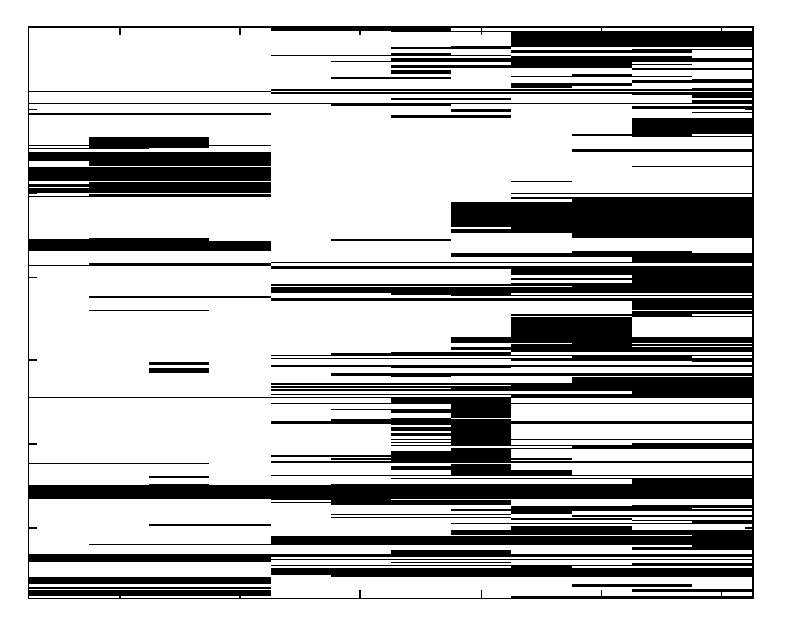
\includegraphics[width=0.8\textwidth]{figures/data}
\end{figure}


\end{frame}

%%%%%%%%%%%%%%%%%%%%%%%%%%%%%%%%%%%%%%%%%%%%%%%%%%%%%%%%%%%%%%%%%%%%%%%%%%%%%%%%%%%%%%%%%%%%%

\begin{frame}{Multiresolution Mixture Modelling Algorithm}
\begin{itemize}
 \item Finite Mixture Models of the Multivariate Bernoulli Distributions  for 0-1 Data\\  
    \vspace{0.1cm}  
\textcolor{blue} { $ P(x) = \sum _{j=1}^{J} \pi _{j} P(x|\theta _{j}) = \sum _{j=1}^{J} \pi _{j} \prod _{i=1}^{d} \theta_{ji}^{x_i}(1-\theta _{ji})^{1-x_{i}}$ } \\
 \scriptsize \item What is done?

\vspace{-1mm}
\begin{figure}
\centering
  \includegraphics[trim=1.2cm 0cm 0cm 1cm, clip=true,width=0.72\textwidth]{figures/idasecondpage}
\end{figure}
\vspace{-5mm}
\scriptsize
\item How is it done?
\item Fast approximation of KL divergence (P. R. Adhikari, J. Hollm\'en, DS 2012) \\ %\textcolor {red} {($\approx 10000$ times faster)}
\scriptsize
\textcolor{blue} {$KL  =  \displaystyle \sum_{i \in X^{*}} \pi_{\alpha} \displaystyle
\prod _{m=1}^{{d}}
\left(\alpha_m^{X^{*}_{im}}(1-\alpha_{m})^{(1-X^{*}_{im})} \right) -
\displaystyle \sum_{i{\prime} \in Y^{*}} \pi_{\beta} \displaystyle \prod
_{n=1}^{{d^{\prime}}} \left(
\beta_{n}^{Y^{*}_{i{\prime}n}}(1-\beta_{n})^{(1-Y^{*}_{i{\prime}n})} \right)
$}
\normalsize \item Retrain the mixture models in different resolutions
\end{itemize}
\end{frame}

%%%%%%%%%%%%%%%%%%%%%%%%%%%%%%%%%%%%%%%%%%%%%%%%%%%%%%%%%%%%%%%%%%%%%%%%%%%%%%%%%%%%%%%%%%%%%
% 
% \begin{frame}{Merging Parameters with different dimensionality}
% \vspace{-2mm}
% \begin{figure}
% \centering
%   \includegraphics[width=\textwidth]{figures/twoformerging}
% \end{figure}
% \end{frame}
%%%%%%%%%%%%%%%%%%%%%%%%%%%%%%%%%%%%%%%%%%%%%%%%%%%%%%%%%%%%%%%%%%%%%%%%%%%%%%%%%%%%%%%%%%%%%

% \begin{frame}{Positive Effect of Minimizing the KL Divergence}
% \vspace{-2mm}
% \begin{figure}
% \centering
%   \includegraphics[width=0.8\textwidth]{figures/iterinem}
% \end{figure}
% \end{frame}

%%%%%%%%%%%%%%%%%%%%%%%%%%%%%%%%%%%%%%%%%%%%%%%%%%%%%%%%%%%%%%%%%%%%%%%%%%%%%%%%%%%%%%%%%%%%%


\begin{frame}{Performance of Multiresolution Mixture Model}
\vspace{-8mm}
\begin{figure}
\centering
  \includegraphics[trim=1.2cm 0cm 0cm 1cm, clip=true, width=1.05\textwidth]{figures/nbarlkhood}  
\end{figure}

\vspace{-10mm}

\scriptsize \hspace{15mm} Better generalization through multiresolution mixture models
\end{frame}

%%%%%%%%%%%%%%%%%%%%%%%%%%%%%%%%%%%%%%%%%%%%%%%%%%%%%%%%%%%%%%%%%%%%%%%%%%%%%%%%%%%%%%%%%%%%%

\begin{frame}{Summary and Conclusions}

\begin{itemize} \setlength{\itemsep}{5.5mm}
 \item The sources of multiresolution data
 \item Multiresolution mixture modelling using merging of mixture components
 \item Fast approximation of KL divergence as the criterion to merge the components
 \item Better generalization over single resolution mixture models
\end{itemize}
\end{frame}

%%%%%%%%%%%%%%%%%%%%%%%%%%%%%%%%%%%%%%%%%%%%%%%%%%%%%%%%%%%%%%%%%%%%%%%%%%%%%%%%%%%%%%%%%%%%%


\begin{frame}
 \frametitle{Thanks, Questions, Comments and Feedback}
 \begin{figure}[h!]
 \centering
 \includegraphics[width=0.5\textwidth]{figures/thanks}
 \end{figure}
 
 \end{frame}
 
%%%%%%%%%%%%%%%%%%%%%%%%%%%%%%%%%%%%%%%%%%%%%%%%%%%%%%%%%%%%%%%%%%%%%%%%%%%%%%%%%%%%%%%%%%%%%
\end{document}
